\documentclass[
    DIV=11,
    BCOR=0mm,
    paper=a4,
    fontsize=11pt,
    % parskip=half,
    twoside=false,
    titlepage=true
% ]{scrreprt}
]{scrartcl}


% -- The basics
\setlength{\parskip}{0.5em} % What parskip=half would do in document class
\setlength{\parindent}{1em} % What would be indent if no parskip given in documentclass
% Set things manually, then we can have indent+skip

\usepackage[left=1in,right=1in,top=0.5in,bottom=1in]{geometry}
\usepackage{graphicx}
\usepackage[utf8]{inputenc}
\usepackage[ngerman, english]{babel}
\usepackage[expansion=true, protrusion=true]{microtype}


% -- Page setup
\usepackage[singlespacing]{setspace} 
\usepackage[automark, headsepline]{scrlayer-scrpage}
\clearmainofpairofpagestyles
\setlength{\headheight}{\baselineskip}
\automark{section} % write section in footline instead of chapter (if there is one)
\automark*{subsection}
\ihead{Max Melching \hfill \headmark}
\usepackage{lastpage}
\cfoot{{\hypersetup{linkcolor=black}Page~\thepage~of~\pageref{LastPage}}}


% -- Link setup
\usepackage{xcolor}
\definecolor{linkblue}{rgb}{0.00,0.00,1.00}

\usepackage{hyperref}
\hypersetup{
    colorlinks=true,
    breaklinks=true,
    citecolor=linkblue,
    linkcolor=linkblue,
    menucolor=linkblue,
    urlcolor=linkblue
}


% -- Font preferences
\usepackage{newtxmath}
\usepackage{tgpagella}
% \setkomafont{chapter}{\rmfamily\Huge\bfseries}
\setkomafont{section}{\rmfamily\Large\bfseries}
\setkomafont{subsection}{\rmfamily\large\scshape}
\setkomafont{paragraph}{\rmfamily}
\setkomafont{title}{\bfseries}
\setkomafont{subtitle}{\Large\scshape}
\setkomafont{author}{\Large\slshape}
\setkomafont{pagehead}{\scshape}
\setkomafont{pagefoot}{\slshape}


% -- Choose special color and font for code bits
\definecolor{codecolor}{RGB}{235, 66, 0}
\newcommand{\code}[1]{\textcolor{codecolor}{\texttt{#1}}}


% -- Customizing itemize labels
\renewcommand{\labelitemi}{$\blacktriangleright$}%{$\vartriangleright$}
\renewcommand{\labelitemii}{\textbf{--}} % is also default there
\renewcommand{\labelitemiii}{$\bullet$}
\setlength{\itemsep}{10pt}


% -- Retrieving git hash
\usepackage{xstring}
\usepackage{catchfile}
\CatchFileDef{\HEAD}{.git/refs/heads/main}{}
\newcommand{\gitrevision}{%
  \StrLeft{\HEAD}{7}%
}
% \CatchFileDef{\TAG}{.git/refs/tags}{}


% -- Some convenience features
\usepackage{siunitx}
\RequirePackage{wasysym}  % For \ascnode symbol


% -- Some custom commands
\newcommand{\defaultval}[1]{%
    {\bfseries\slshape%\itshape
    % Default:} #1%
    Default} $=$ #1%
}



\begin{document}

% \chapter*{Documentation Of \code{GWFrames}}
{\rmfamily\Huge\bfseries
    Documentation Of \code{GWFrames}
}

For the most recent version of all the files, see \url{https://github.com/MaxMelching/gw_frames}.
This file was compiled on \today{} and the corresponding git commit hash
is \code{\gitrevision{}} (or, in case you need the full one, \code{\HEAD{}}\hspace{-0.5em}).



    \section{Overview}

This repository contains three packages, each providing one command:
\begin{itemize}
    \item \code{cbc\_frames\_tikz} (command \verb|\drawframes|): plots a
    selection of source frame, signal frame, and celestial frame that are
    used to describe gravitational waves emitted by compact binary coalescences.
    
    
    \item \code{cbc\_binary\_tikz} (command \verb|\drawbinary|): plots
    intrinsic parameters of a system of two compact binary objects. Adapted
    from code originally written by Jannik Mielke.
    
    
    \item \code{earth\_tikz} (command \verb|\drawearth|): plots one side of
    the Earth. Mainly intended for usage through \verb|\drawframes|. Most of
    the credit for this code goes to Izaak Neutelings, who provided it on
    \url{https://tikz.net/astronomy_seasons/}.
\end{itemize}

Several examples of how to use this package are shown in the examples folder.
% Pictures are also included in Fig.~\ref{fig:examples}.

% \begin{figure}[h]
%     \centering

%     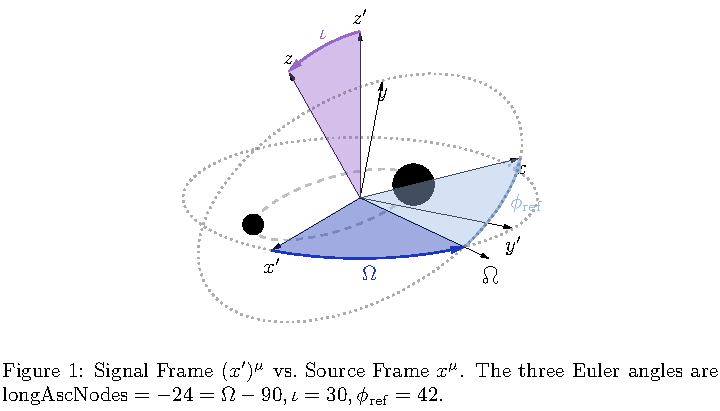
\includegraphics[width=0.67\textwidth]{examples/signal_frame.pdf}
%     \label{fig:examples}
% \end{figure}



    \section{List Of Keyword Arguments}

\emph{Note} that certain values cannot be passed to pgfkeys, which is
particularly relevant for declaration of labels. If you encounter an issue of
this kind, look up the command that this key is stored in (typically something
like \verb|\<parameter>Label|), and manually set the command. This can be done
using \verb|\def\<parameter>Label{<input>}|. A practical example would be
\verb|\def\OmegaLabel{$\Omega = \pi/2 + \mathrm{longAscNodes}$}|.


        \subsection{\texttt{cbc\_frames\_tikz}}

This is a list of all keyword arguments (note that all angles are expected to
be given in degrees):
\begin{itemize}
    \item \code{mass1}: mass of the first compact object, determining its
    size. Ten solar masses correspond to a size of $\SI{0.35}{\centi\metre}$.
    
    \defaultval{$20$}


    \item \code{mass2}: mass of the second compact object, determining its
    size. Ten solar masses correspond to a size of $\SI{0.35}{\centi\metre}$.
    
    \defaultval{$20$}
    
    
    \item \code{longascnodes}: determines the angle between $x$-axis of the
    signal frame and the ascending node $\ascnode$, this angle being
    $\Omega = 90 + \mathrm{longAscNodes}$.
    
    \defaultval{$0$}


    \item \code{inclination}: inclination between orbital plane and sky plane.
    This rotation is about the ascending node $\ascnode$.
    
    \defaultval{$0$}
    
    
    \item \code{phiref}: reference angle $\phi_\mathrm{ref}$ that determines
    the rotation between ascending node and $x$-axis of the signal frame
    (about the inclined $z$-axis of the signal frame).
    
    \defaultval{$0$}
    
    
    \item \code{ra}
    
    
    \item \code{dec}
    
    
    \item \code{polarization}: polarization angle, i.e. rotation of the $x$-axis
    in the sky plane (about the line of sight).


    \item \code{eccentricity}


    \item \code{axislen}: length of the axes in each coordinate system.
    
    \defaultval{$\SI{3}{\centi\metre}$}


    \item \code{binaryscalefactor}: distance of binary companions, in multiples
    of the axis length \code{axislen}.
    
    \defaultval{$1$}


    \item \code{binarydistance}: distance of binary center of mass from Earth,
    in multiples of the axis length \code{axislen}.
    
    \defaultval{$3$}


    % \item \code{uselayers}


    \item \code{showcelestialframe}: determines whether to show the celestial frame.
    Has precedence over the other commands for styling of celestialframe, such
    as \code{celestialframeaxes}.

    \defaultval{true}


    \item \code{celestialframeaxes}


    \item \code{celestialframehelperlines}


    \item \code{celestialframeangles}


    \item \code{showlineofsight}


    \item \code{showsignalframe}: determines whether to show the signal frame.
    Has precedence over the other commands for styling of signalframe, such
    as \code{signalframeaxes}.

    \defaultval{true}


    \item \code{signalframeaxes}


    \item \code{signalframehelperlines}


    \item \code{signalframeangles}


    \item \code{showsourceframe}


    \item \code{sourceframeaxes}


    \item \code{sourceframehelperlines}


    \item \code{earthradius}


    \item \code{earthtilt}: 


    \item \code{showifo}: whether to draw an interferometer on Earth or not.


    \item \code{ifoarmlength}: arm length of the interferometer.
    
    \defaultval{$\SI{2}{\centi\metre}$}
\end{itemize}


        \subsection{\texttt{cbc\_binary\_tikz}}


        \subsection{\texttt{earth\_tikz}}


\end{document}